\subsection{Уравнение колебаний полубесконечной струны (стержня). Метод отражений.}

%\begin{equation}
	%\square_{a} = \frac{\partial^2}{\partial t^2} - a^2 \Delta
%\end{equation}

Изложенный в пункте \ref{DalamberFormula} метод решения задачи Коши позволяет решать некоторые смешанные задачи для этого уравнения. Для определенности рассмотрим смешанную задачу, описыващую колебание полубесконечной струны $x > 0$ с закрепленным левым концом \footnote{Все взято из Владимирова - стр. 187 и далее}
\begin{equation} \label{x0cond}
	u |_{x = 0} = 0.
\end{equation}

Предварительно докажем, что всякое классическое решение $u(x, t)$ уравнения \eqref{infinite_string} в квадрате $x > 0$, $t > 0$, удовлетворяющее условию \eqref{x0cond} представляется в виде 
\begin{equation} \label{xg0condim}
	u(x, t) = g(x + a t) - g(-x + a t)
\end{equation}
(т.к. подставляя начальные условия в \eqref{general_int} $0 = f_1(-a t) + f_2(a t)$
отсюда и вытекает представление \eqref{xg0condim}).

Построим решение смешанной задачи \eqref{infinite_string}, \eqref{inf_str_cond}, \eqref{x0cond}. Всякое классическое решение $u(x, t)$ этой задачи в силу \eqref{xg0condim} допускает нечетное продолжение $\tilde{u}(x, t)$ по $x$ класса $\mathcal{C}^2(\mathbb{R}^2)$, и это продолжение удовлетворяет уравнению \eqref{infinite_string} в $\mathbb{R}^2$.
\begin{figure}[H]
	\centering
	\begin{subfigure}{0.4\textwidth}
		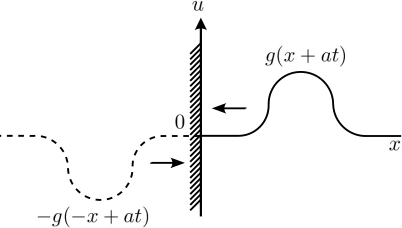
\includegraphics[width=\textwidth]{img/mirror1.png}
		\caption{}
	\end{subfigure}
	\hspace{5mm}
	\begin{subfigure}{0.4\textwidth}
		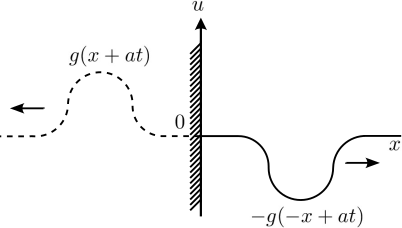
\includegraphics[width=\textwidth]{img/mirror2.png}
		\caption{}
	\end{subfigure}
	\caption{}
\end{figure}
Отсюда из условий \eqref{inf_str_cond} вытекает, что решение $\tilde{u}(x, t)$ удовлетворяет начальным условиям
\begin{equation}
	\tilde{u}|_{t = 0} = \tilde{u}_0(x), \quad \tilde{u}_t|_{t = 0} = \tilde{u}_1(x),
\end{equation}
где $\tilde{u}_0$ и $\tilde{u}_1$ --- нечетные продолжения функций $u_0$ и $u_1$ соответственно. Но решение такой задачи Коши единственно и представляется формулой Даламбера \eqref{dAlamber} с заменой $u_0$ на $\tilde{u}_0$ и $u_1$ на $\tilde{u}_1$, если $\tilde{u}_0 \in \mathcal{C}^2(\mathbb{R}^1)$ и $\tilde{u}_1 \in \mathcal{C}^1(\mathbb{R}^1)$. Последние условия будут выполнены, если
\begin{equation} \label{setcond}
	u_0 \in \mathcal{C}^2(x \geqslant 0), \quad u_1 \in \mathcal{C}^1(x \geqslant 0), \quad u_0(0) = u_0''(0) = u_1(0) = 0.
\end{equation}

Итак, если выполнены условия \eqref{setcond}, то решение задачи \eqref{infinite_string}, \eqref{inf_str_cond}, \eqref{x0cond} существует, единственно и задается формулой 
\begin{equation} \label{formula}
	u(x, t) = \frac{1}{2} [\tilde{u}_0(x + a t) + \tilde{u}_0(x - a t)] + \frac{1}{2 a} \int_{x - a t}^{x + a t} \tilde{u}_1(\xi) \, d\xi, \quad x \geqslant 0.
\end{equation}

Пусть $x - a t \geqslant 0$. Тогда
\begin{equation}
	\tilde{u}_0(x - a t) = \tilde{u}_0(x - a t), \quad \tilde{u}_1(\xi) = u_1(\xi), \quad \xi \geqslant x - a t \geqslant 0,
\end{equation}
и формула \eqref{formula} принимает вид 
\begin{equation}
	u(x, t) = \frac{1}{2} [u_0(x + a t) + u_0(x - a t)] + \frac{1}{2 a} \int_{x - a t}^{x + a t} u_1(\xi) \, d\xi, \quad x \geqslant at.
\end{equation}

Аналогичные рассуждения можно провести для $x - a t \leqslant 0$. 
\begin{equation*}
	\tilde{u}_0(x - a t) = - u_0(-x + a t), \quad \tilde{u}_1(\xi) = -u_1(-\xi), \quad x - a t \leqslant \xi \leqslant 0,
\end{equation*}
формула \eqref{formula} принимает вид
\begin{equation} \label{other_formula}
	u(x, t) = \frac{1}{2} [u_0(x + a t) - u_0(-x + a t)] + \frac{1}{2a} \int_{-x + a t}^{x + a t} u_1(\xi) \,d\xi, \quad 0 \leqslant x \leqslant a t.
\end{equation}

Как видно из формулы \eqref{other_formula}, в точку $(x, t)$, $0 \leqslant x \leqslant a t$, приходят два волны: прямая волна из точки $(x + a t, 0)$ и один раз отраженная волна из точки $(a t - x, 0)$ (совпадающая с прямой волной из фиктивной точки $(x - at, 0)$; см. рис. 2).

\begin{figure}[H]
	\centering
	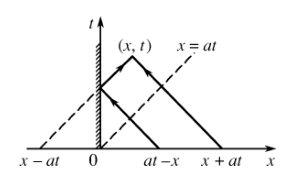
\includegraphics[width=0.4\linewidth]{img/mirror3}
	\caption{}
\end{figure}

Аналогично рассматривается смешанная задача для полубесконечной струны $x > 0$ со свободным концом:
\begin{equation*}
	u_x|_{x = 0} = 0.
\end{equation*}
Здесь также имеет место отражение волн от конца струны $x = 0$, но уже без изменения знака. 
